\documentclass[10pt]{article}
\usepackage[a4paper,landscape,margin=0.18in]{geometry}
\usepackage[utf8]{inputenc}
\usepackage{tikz}
\usepackage{amsmath}
\usepackage{pifont}
\usepackage{helvet}
\usepackage{array}
\usepackage{tabularx}
\usetikzlibrary{arrows.meta,positioning,fit,calc}

\renewcommand{\familydefault}{\sfdefault}
\pagestyle{empty}

\definecolor{indigo}{RGB}{54,40,145}
\definecolor{deepblue}{RGB}{30,48,125}
\definecolor{lineblue}{RGB}{113,160,225}
\definecolor{lightblue}{RGB}{239,247,255}
\definecolor{lightpurple}{RGB}{243,240,255}
\definecolor{green}{RGB}{20,135,93}
\definecolor{lightgreen}{RGB}{231,249,241}
\definecolor{red}{RGB}{220,60,63}
\definecolor{lightred}{RGB}{255,238,239}
\definecolor{gold}{RGB}{246,184,64}

\newcommand{\cmark}{\textcolor{green}{\ding{51}}}
\newcommand{\xmark}{\textcolor{red}{\ding{55}}}
\newcommand{\panel}[4]{%
  \node[draw=lineblue, rounded corners=5pt, line width=.8pt, fill=white,
        inner sep=6pt, text width=#2, minimum height=#3, anchor=north west] (#1) at #4 {};}
\newcommand{\headerbar}[3]{%
  \node[fill=indigo, text=white, rounded corners=3pt, anchor=north west,
        minimum width=#2, minimum height=0.28in, align=left, inner xsep=7pt,
        font=\bfseries\large] at #3 {#1};}
\newcommand{\smallbullet}{\textcolor{deepblue}{\large\textbullet}\hspace{2pt}}

\begin{document}
\resizebox{11.25in}{!}{%
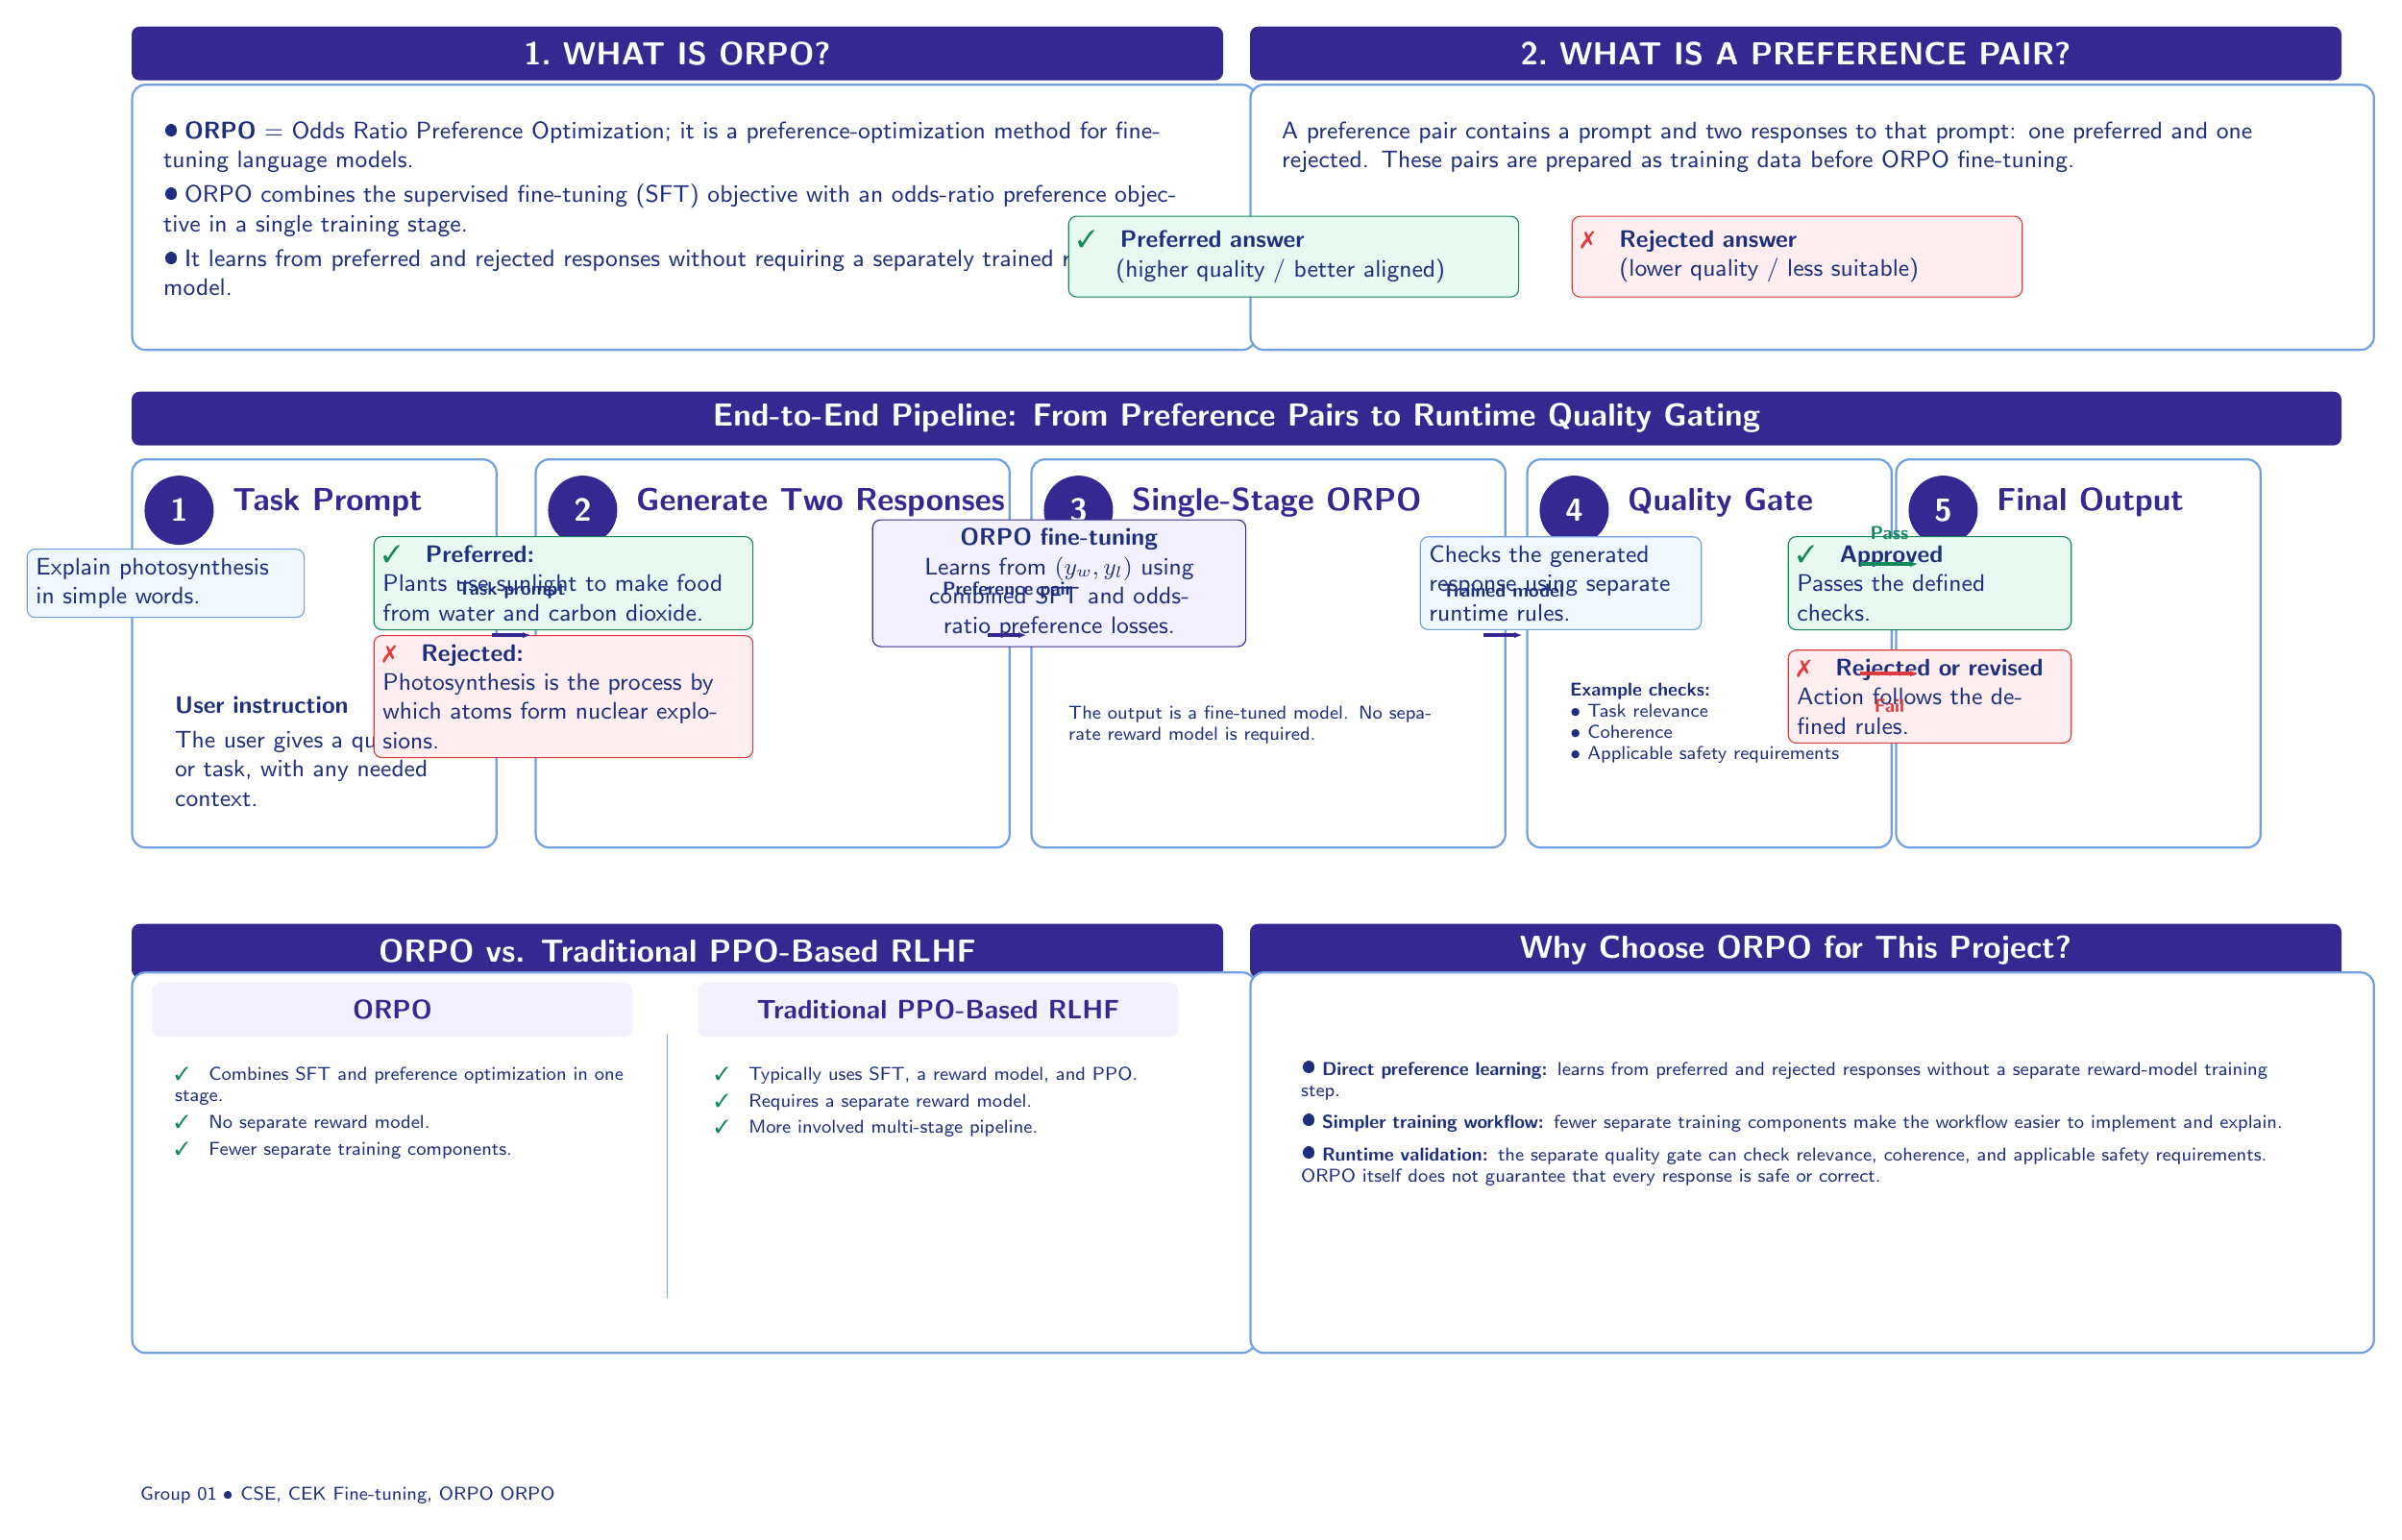
\begin{tikzpicture}[x=1in,y=1in]
\sffamily

% Top definition panels
\headerbar{1.\ WHAT IS ORPO?}{5.68in}{(0,7.92in)}
\panel{defone}{5.68in}{1.38in}{(0,7.62in)}
\node[anchor=north west, text width=5.35in, align=left, font=\small, text=deepblue] at (0.12,7.47) {
\smallbullet \textbf{ORPO} = Odds Ratio Preference Optimization; it is a preference-optimization method for fine-tuning language models.\\[2pt]
\smallbullet ORPO combines the supervised fine-tuning (SFT) objective with an odds-ratio preference objective in a single training stage.\\[2pt]
\smallbullet It learns from preferred and rejected responses without requiring a separately trained reward model.};

\headerbar{2.\ WHAT IS A PREFERENCE PAIR?}{5.68in}{(5.82in,7.92in)}
\panel{deftwo}{5.68in}{1.38in}{(5.82in,7.62in)}
\node[anchor=north west, text width=5.3in, align=left, font=\small, text=deepblue] at (5.94,7.47) {A preference pair contains a prompt and two responses to that prompt: one preferred and one rejected. These pairs are prepared as training data before ORPO fine-tuning.};
\node[draw=green, fill=lightgreen, rounded corners=3pt, text width=2.25in, minimum height=.42in, align=left, font=\small, text=deepblue] at (6.05,6.72) {\cmark\quad \textbf{Preferred answer}\\\hspace{.2in}(higher quality / better aligned)};
\node[draw=red, fill=lightred, rounded corners=3pt, text width=2.25in, minimum height=.42in, align=left, font=\small, text=deepblue] at (8.67,6.72) {\xmark\quad \textbf{Rejected answer}\\\hspace{.2in}(lower quality / less suitable)};

% Pipeline title
\headerbar{End-to-End Pipeline: From Preference Pairs to Runtime Quality Gating}{11.5in}{(0,6.02in)}

% Pipeline cards
\panel{p1}{1.73in}{2.02in}{(0,5.67in)}
\node[fill=indigo, text=white, circle, minimum size=.36in, font=\bfseries\large] at (.25,5.40) {1};
\node[anchor=north west, font=\bfseries\large, text=indigo] at (.48,5.56) {Task Prompt};
\node[draw=lineblue, fill=lightblue, rounded corners=3pt, text width=1.35in, align=left, font=\small, text=deepblue] at (.18,5.02) {Explain photosynthesis in simple words.};
\node[anchor=north west, text width=1.42in, align=left, font=\small, text=deepblue] at (.18,4.48) {\textbf{User instruction}\\[2pt]The user gives a question or task, with any needed context.};

\panel{p2}{2.30in}{2.02in}{(2.10in,5.67in)}
\node[fill=indigo, text=white, circle, minimum size=.36in, font=\bfseries\large] at (2.35,5.40) {2};
\node[anchor=north west, font=\bfseries\large, text=indigo] at (2.58,5.56) {Generate Two Responses};
\node[draw=green, fill=lightgreen, rounded corners=3pt, text width=1.88in, align=left, font=\small, text=deepblue] at (2.25,5.02) {\cmark\quad \textbf{Preferred:}\\Plants use sunlight to make food from water and carbon dioxide.};
\node[draw=red, fill=lightred, rounded corners=3pt, text width=1.88in, align=left, font=\small, text=deepblue] at (2.25,4.43) {\xmark\quad \textbf{Rejected:}\\Photosynthesis is the process by which atoms form nuclear explosions.};

\panel{p3}{2.30in}{2.02in}{(4.68in,5.67in)}
\node[fill=indigo, text=white, circle, minimum size=.36in, font=\bfseries\large] at (4.93,5.40) {3};
\node[anchor=north west, font=\bfseries\large, text=indigo] at (5.16,5.56) {Single-Stage ORPO};
\node[draw=indigo, fill=lightpurple, rounded corners=3pt, text width=1.85in, align=center, font=\small, text=deepblue] at (4.83,5.02) {\textbf{ORPO fine-tuning}\\Learns from $(y_w,y_l)$ using combined SFT and odds-ratio preference losses.};
\node[anchor=north west, text width=1.92in, align=left, font=\scriptsize, text=deepblue] at (4.83,4.43) {The output is a fine-tuned model. No separate reward model is required.};

\panel{p4}{1.73in}{2.02in}{(7.26in,5.67in)}
\node[fill=indigo, text=white, circle, minimum size=.36in, font=\bfseries\large] at (7.51,5.40) {4};
\node[anchor=north west, font=\bfseries\large, text=indigo] at (7.74,5.56) {Quality Gate};
\node[draw=lineblue, fill=lightblue, rounded corners=3pt, text width=1.37in, align=left, font=\small, text=deepblue] at (7.44,5.02) {Checks the generated response using separate runtime rules.};
\node[anchor=north west, text width=1.4in, align=left, font=\scriptsize, text=deepblue] at (7.44,4.55) {\textbf{Example checks:}\\$\bullet$ Task relevance\\$\bullet$ Coherence\\$\bullet$ Applicable safety requirements};

\panel{p5}{1.73in}{2.02in}{(9.18in,5.67in)}
\node[fill=indigo, text=white, circle, minimum size=.36in, font=\bfseries\large] at (9.43,5.40) {5};
\node[anchor=north west, font=\bfseries\large, text=indigo] at (9.66,5.56) {Final Output};
\node[draw=green, fill=lightgreen, rounded corners=3pt, text width=1.38in, align=left, font=\small, text=deepblue] at (9.36,5.02) {\cmark\quad \textbf{Approved}\\Passes the defined checks.};
\node[draw=red, fill=lightred, rounded corners=3pt, text width=1.38in, align=left, font=\small, text=deepblue] at (9.36,4.43) {\xmark\quad \textbf{Rejected or revised}\\Action follows the defined rules.};

% Arrows
\foreach \x/\label in {1.88/{Task prompt},4.46/{Preference pair},7.04/{Trained model}} {
  \draw[-{Latex[length=3pt]}, very thick, indigo] (\x,4.75) -- ++(.20,0);
  \node[font=\scriptsize\bfseries, text=deepblue, align=center] at (\x+.10,4.98) {\label};
}
\draw[-{Latex[length=3pt]}, very thick, green] (9.00,5.12) -- (9.30,5.12);
\node[font=\scriptsize\bfseries, text=green] at (9.15,5.28) {Pass};
\draw[-{Latex[length=3pt]}, very thick, red] (9.00,4.55) -- (9.30,4.55);
\node[font=\scriptsize\bfseries, text=red] at (9.15,4.38) {Fail};

% Bottom comparison and selection panels
\headerbar{ORPO vs. Traditional PPO-Based RLHF}{5.68in}{(0,3.25in)}
\panel{compare}{5.68in}{1.98in}{(0,3.00in)}
\node[fill=lightpurple, rounded corners=3pt, text=indigo, font=\bfseries, minimum width=2.50in, minimum height=.28in] at (1.36,2.80) {ORPO};
\node[fill=lightpurple, rounded corners=3pt, text=indigo, font=\bfseries, minimum width=2.50in, minimum height=.28in] at (4.20,2.80) {Traditional PPO-Based RLHF};
\node[anchor=north west, text width=2.48in, align=left, font=\scriptsize, text=deepblue] at (.18,2.55) {\cmark\quad Combines SFT and preference optimization in one stage.\\[2pt] \cmark\quad No separate reward model.\\[2pt] \cmark\quad Fewer separate training components.};
\node[anchor=north west, text width=2.48in, align=left, font=\scriptsize, text=deepblue] at (2.99,2.55) {\cmark\quad Typically uses SFT, a reward model, and PPO.\\[2pt] \cmark\quad Requires a separate reward model.\\[2pt] \cmark\quad More involved multi-stage pipeline.};
\draw[lineblue] (2.79,2.67) -- (2.79,1.30);

\headerbar{Why Choose ORPO for This Project?}{5.68in}{(5.82in,3.25in)}
\panel{why}{5.68in}{1.98in}{(5.82in,3.00in)}
\node[anchor=north west, text width=5.24in, align=left, font=\scriptsize, text=deepblue] at (6.04,2.58) {\smallbullet \textbf{Direct preference learning:} learns from preferred and rejected responses without a separate reward-model training step.\\[4pt]
\smallbullet \textbf{Simpler training workflow:} fewer separate training components make the workflow easier to implement and explain.\\[4pt]
\smallbullet \textbf{Runtime validation:} the separate quality gate can check relevance, coherence, and applicable safety requirements. ORPO itself does not guarantee that every response is safe or correct.};

\node[anchor=south west, font=\scriptsize, text=deepblue] at (0,.18) {Group 01 \textbullet\ CSE, CEK \hfill Fine-tuning, ORPO \hfill ORPO};
\end{tikzpicture}%
}
\end{document}
